\documentclass[12pt,a4paper]{article}

% Türkçe %
\usepackage[utf8]{inputenc} %Türkçe karakterler için
\usepackage[T1]{fontenc}
\renewcommand{\tablename}{Tablo}
\renewcommand{\figurename}{Şekil}
\renewcommand{\indexname}{Dizin}
\renewcommand{\listfigurename}{Şekiller}
\renewcommand{\listtablename}{Tablolar}
\renewcommand{\contentsname}{İçindekiler}
\setcounter{tocdepth}{4}
\setcounter{secnumdepth}{4}
% Türkçe %

\usepackage{geometry}
\usepackage{graphicx} %Resim koymak için
\usepackage{times} %Times fontu
\usepackage[nottoc]{tocbibind}
\usepackage{url}
\usepackage{array}
\usepackage{tabu}

\begin{document}
   \pagenumbering{gobble}
   \begin{titlepage}
   \begin{center}
      \begin{large}
         \vspace*{0.5cm}
         GAZİ ÜNİVERSİTESİ \\
         MÜHENDİSLİK FAKÜLTESİ \\
         BİLGİSAYAR MÜHENDİSLİĞİ

         \vfill
         BM 314 YAZILIM MÜHENDİSLİĞİ \\
         SPMP BELGESİ

         \vfill
         Abdullah Akalın\\Bekir Aydın\\Karim El Guermai\\Muhammed Emre Emrah\\

         \vfill
         \vspace{0.5cm}
         24.03.1017
      \end{large}
   \end{center}
\end{titlepage}

   \newpage

   \pagenumbering{roman}
   \tableofcontents
   \newpage

   \pagenumbering{arabic}

   \section{KAPSAM}
   \subsection{Tanım} \label{kaps}
   Bu belge yazılım gereksinim dökümanıdır. Gerçekleştirilecek oyun projesinin gereksinimleri ayrıntılı biçimde sunulacaktır. Belgede \textit{"Karakter"}, oyuncunun yönettiği oyun karakterini temsil etmektedir. \textit{Düşman}, karakterin kendisine çarptığında ceza durumuna düştüğü yardımcı karakterdir. \textit{"Merdiven"}, oyunun arkaplanında bulunacak ve karakterin esas hareket alanı olan zemini temsil etmektedir. \textit{"Harf"}, karakterin merdivenler üzerinde basamaklarda bulunan harfleri temsil etmektedir. Oyuncu bu harfleri toplayarak kelimeyi tamamlamaya çalışır. \textit{"Sahne"}, oyuncunun oyunu oynadığı ekran için kullanılacaktır. \textit{"Kelime göstergesi"}, sahnenin üst kısmında bulunacak olan tamamlanacak kelimenin tamamlanma durumunu gösteren görseldir. \textit{Puan ve Puan Göstergesi} sırasıyla, oyuncunun aşağıda belirtilen yollarla kazandığı puanı ve sahnenin üst kısmında bulunacak olan toplanan puanların yekününün gösterildiği görsele işaret etmektedir. Bunların yanısıra \textit{"Mobil cihaz"} ile oyunun oynanacağı fiziksel cihaz, \textit{"Geliştirme ortamı"} ile oyunun geliştirildiği bilgisayar ortamı ifade edilmektedir. Ayrıca \textit{"SPMP"} kısaltması, tarafımızdan müşteriye sunulan proje yönetim planı belgesini ifade etmektedir.

   \subsection{Genel Bakış} \label{genel}
   Bu oyunda, oyuncu küçük uykulu bir kahve çekirdeğini yönetecektir. Oyun merdivenlerin olduğu bir sahnede geçmektedir ve merdivenlerin en alt basamağında karakterin yatağı bulunmaktadır. Karakter devamlı aşağı inip yatağına ulaşmak istemektedir. Oyuncu ise ona, merdivenlerde bulunan harfleri toplatıp bölümü geçmek için gerekli olan kelimeyi tamamlatmak suretiyle bölümü tamamlatmak istemektedir. Ayrıca merdiven başlarından çıkan düşmanlara çarpılması halinde karakter harf kaybedecektir. Sahip olduğu tüm harfleri kaybetmesi halinde ise yanacaktır. Oyunun sonunda skor görüntülenecek ve oyuncu her defasında oyuna baştan başlayıp her seferinde ulaşabildiği kadar ilerideki kelimelere ulaşmaya çalışacaktır.
   Sistemin kullanıcıları genç ve yetişkin oyunculardır. Bu durum, sistemin esnek bir şekilde geliştirilmesine olanak sağlamaktadır. Oyunun ana gayesi oyuncuya eğlenceli vakit geçirmektir.

   \subsection{Dokümana Genel Bakış}
   Bu belge IEEE/ANSI 830-1998\footnote{http://standards.ieee.org/findstds/standard/830-1998.html} standardını takip etmektedir ve geliştirilen sistemin kullanıcı ve sistem gereksinimlerini tanımlamaktadır. Dökümanın kullanımında, bu sistemin bir mobil oyun olduğu göz önünde bulundurulmalıdır. Bunun dışında belgeyle ilgili özel bir husus bulunmamaktadır.

   \section{İLGİLİ DOKÜMANLAR}
   Bu belgede müşteriye daha önce tarafımızdan sunulan SPMP belgesine atıfta bulunulmuştur.
   \begin{itemize}
      \item Başlık: SPMP, Revizyon: 1, Tarih: 24.03.2017
   \end{itemize}

   \section{GEREKSİNİMLER}
   Gereksinimler, alt başlıklar halinde aşağıda belirtilmiştir. Tüm gereksinimlerin içerildiği akış şeması için Ek--\ref{fc} bölümüne müracaat ediniz.

   \subsection{Gerekli Durum ve Modlar}
   Bu sistem özel durum ve modlar bulunmamaktadır.

   \subsection{YKE Fonksiyonel Gereksinimleri} \label{ger}

   \subsubsection{Menü Seçimi}
   \begin{figure}
      \begin{center}
         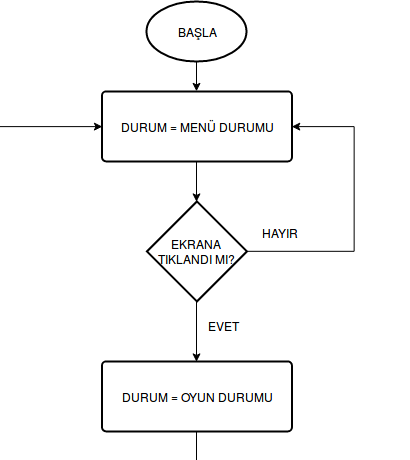
\includegraphics{res/menu.png}
         \caption{Menü seçim gereksinimi akış şeması}
         \label{fig:menu}
      \end{center}
   \end{figure}
   Oyuncu oyuna başladığında karşısına sade bir menü gelecektir. Menünün ekranda bulunan tek bir düğmeden oluşması planlanmaktadır. Kullanıcının düğmeye tıklaması halinde oyun başlayacak, tıklamaması halinde bekleyecektir. Oyuncu cihazında bulunan "geri" tuşuyla uygulamadan çıkabilecektir. Bu durum Şekil \ref{fig:menu} üzerinde resmedilmiştir.

   \subsubsection{Merdiven Çıkma/İnme}
   \begin{figure}[h!]
      \begin{center}
         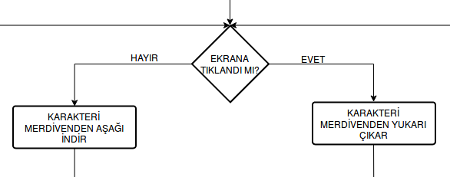
\includegraphics{res/st.png}
         \caption{Merdiven çıkma/inme diyagramı}
         \label{fig:st}
      \end{center}
   \end{figure}
   Oyuncunun oyun esnasında ekrana dokunmasıyla karakterin merdiveni bir basamak çıkması, dokunmayı kesmesiyle de bir basamak inmesi gerekmektedir. Bu durum Şekil \ref{fig:st} üzerinde görülmektedir.

   \subsubsection{Harf Toplama}
   Oyuncu; karaktere, merdivenleri çıkararak merdiven basamaklarında bulunan harfleri toplatacaktır. Bu harfler ile bölümü geçmek için belirlenmiş kelimeyi tamamlayacaktır. Ayrıca harfleri düşmanlara kaptırmaması gerekmektedir.

   \subsubsection{Karakter--Harf Çarpışması}
   \begin{figure}[h!]
      \begin{center}
         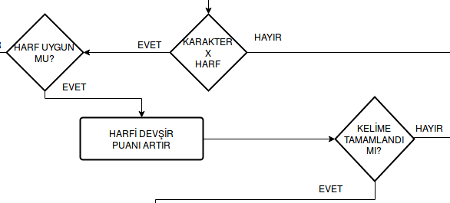
\includegraphics{res/cxl.png}
         \caption{Karakter--Harf çarpışması diyagramı}
         \label{fig:cxl}
      \end{center}
   \end{figure}
   Karakter, harf ile çarpıştığında harf, tamamlaması gereken kelime için uygunsa harfi alacaktır, değilse alamayacaktır. Alınan harfler sahnenin üst kısmında bulunan kelime göstergesinde görüntülenecektir ve puan artırılacaktır. Her harf alımında istenen kelimenin tamamlanıp tamamlanmadığı kontrol edilecektir. Bu gereksinim Şekil \ref{fig:cxl} üzerinde gösterilmiştir.

   \subsubsection{Düşman--Harf Çarpışması}
   \begin{figure}[h!]
      \begin{center}
         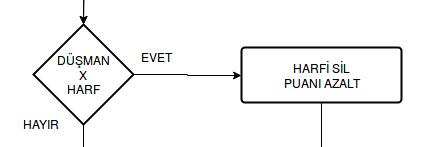
\includegraphics{res/exl.png}
         \caption{Düşman--Harf çarpışması diyagramı}
         \label{fig:exl}
      \end{center}
   \end{figure}
   Düşman, harfe rast geldiğinde onu alır ve karakterin almasına mani olur. Ayrıca oyuncunun puanı düşürülür. Bu durum Şekil \ref{fig:exl} üzerinden gözlenebilir.

   \subsubsection{Karakter--Düşman Çarpışması} \label{ssec:cxe}
   \begin{figure}
      \begin{center}
         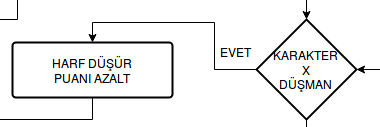
\includegraphics{res/cxe.png}
         \caption{Karakter--Düşman çarpışması diyagramı}
         \label{fig:cxe}
      \end{center}
   \end{figure}
   Karakter ile düşmanın çarpışması durumunda Şekil \ref{fig:cxe} üzerinde görüldüğü üzere, karakter topladığı harflerden bir tane kaybeder ve puan azalır. 

   \subsubsection{Bölüm Geçme}
   Oyuncu kelimeleri tamamlayarak sonraki bölümlere geçip, daha uzun kelimeleri tamamlamaya çalışacaktır. Her bölüm aynı sahnede geçecek olup biribirinin devamı niteliğinde olacaktır.

   \subsubsection{Yanma ve Oyunun Bitmesi}
   Oyuncu düşmanla çarpıştığında (bkz. \ref{ssec:cxe}) harf kaybeder. Eğer hiç harfi kalmamışsa yanar ve oyun biter. Ana menüye dönülür. Benzer şekilde, şayet oyuncu en alt kata kadar inerse oyun biter ve ana menüye dönülür.

   \subsection{YKE Dış Arayüz Gereksinimleri}
   Oyunun oyuncuyla etkileşimi tamamen dokunmatik ekran üzerinden olacaktır. Oyuncunun dokunmasıyla karakter merdivenleri çıkacak, oyuncunun dokunmayı kesmesiyle merdivenleri inecektir. Ayrıca oyuncu menü ekranındaki düğmeye basarak akışı başlatacaktır. (bkz.\ref{ger})

   \subsubsection{Arayüz Tanımlaması ve Diyagramları} \label{ara}
   Oyun temel olarak iki arayüzden oluşacaktır.

   \paragraph{Menü Arayüzü}
   Birincisi menü arayüzüdür. Bu arayüzde sadece bir arkaplan resmi ve bir oyuna başlama düğmesi bulunacaktır. Taslak, Şekil \ref{fig:gm} üzerinde görülebilir.
   \begin{figure}[h!]
      \begin{center}
         
\includegraphics{res/gm.png}
         \caption{Menü arayüzüne ait taslak görüntü.}
         \label{fig:gm}
      \end{center}
   \end{figure}

   \paragraph{Oyun Arayüzü}
   Diğer arayüz ise oyunun oynandığı arayüz olacaktır. Bu arayüzün taslağı, Şekil \ref{fig:gp} üzerinde görülebilir. Ayrıntılı bilgi için \ref{genel} başlığına müracaat ediniz.
   \begin{figure}[h!]
      \begin{center}
         
\includegraphics{res/gp.png}
         \caption{Oyun arayüzüne ait taslak görüntü.}
         \label{fig:gp}
      \end{center}
   \end{figure}

   \subsection{YKE Dahili Arayüz Gereksinimleri}
   Bölüm \ref{ara} içinde belirtildiği üzere oyunda iki arayüz olacaktır. Bu arayüzler için gerekli grafiklerin hazırlanması gerekmektedir. Buna göre,
   \begin{itemize}
      \item Logo
      \item Arkaplan
      \item Düğme
      \item Sahne
      \item Karakter
      \item Harf
      \item Düşman
      \item Kelime göstergesi
      \item Puan
   \end{itemize}
   öğeleri için grafikler hazırlanması gerekmektedir.

   \subsection{YKE Dahili Veri Gereksinimleri}
   Oyunun dahili olarak, bölümler için seçilecek kelimelerden oluşan veri kümesine ihtiyacı vardır.

   \subsection{Uyarlama Gereksinimleri}
   Oyun sadece Android platformunda çalışacaktır ve herhangi bir uyarlama gereksinimi içermeyecektir.

   \subsection{Emniyet Gereksinimleri}
   Uzun süre ekrana bakılması göz sağlığı açısından zararlıdır. Bu yüzden 20 dakikalık aralarla oyuncunun gözlerini dinlendirmesi gerekmektedir.

   \subsection{Güvenlik ve Gizlilik Gereksinimleri}
   Sistem, Google Play Services altyapısını kullanacaktır. 

   \subsection{YKE Ortam Gereksinimleri} \label{ortam}
   Oyun için Android mobil işletim sistemi ile çalışan, dokunmatik yüzeye sahip ve asgari 4.4.4 sürümünü destekleyen herhangi bir cihaz gerekmektedir.

   \subsection{Bilgisayar Kaynak Gereksinimleri}
   \subsubsection{Bilgisayar Donanım Gereksinimleri}
   Donanım gereksinimi bulunmamaktadır.

   \subsubsection{Bilgisayar Donanımı Kaynak Kullanımı Gereksinimleri}
   Cihazın görüntü, ses ve dokunmatik yüzey kaynaklarına sahip olması gerekmektedir.

   \subsubsection{Bilgisayar Yazılım Gereksinimleri}
   Bakınız \ref{ortam}.
   
   \subsubsection{Bilgisayar İletişim Gereksinimleri}
   Oyunun Google Play Services'a bağlanmak için internet bağlantısına ihtiyacı olacaktır.

   \subsection{Yazılım Kalite Faktörleri}
   \paragraph{Erişilebilirlik}
   Oyun, dünya çapında geçerliliği olan Google Play Store'a yüklenecektir. Dolayısıyla erişim kolay olacaktır.
   \paragraph{Uyumluluk}
   Oyunda kullanılan Android API versiyonu sayesinde dünya üzerinde kullanılan Android mobil cihazların \%70'den fazlası ile uyumlu olacaktır\footnote{https://developer.android.com/about/dashboards/index.html}.
   \paragraph{Kullanılabilirlik}
   Oyun, basit arayüzleri ve kolay oynanımı ile kullanılabilir olacaktır.

   \subsection{Tasarım ve Uygulama Kısıtlamaları}
   Sistemin tasarımında Java programlama dili ve libGDX kütüphanesi kullanılacaktır. Geliştiriminde ise Android Studio IDE yazılımı kullanılacaktır.

   \subsection{Personelle İlgili Gereksinimler}
   YKE kullanıcılarının herhangi bir Android işletim sistemli akıllı telefon kullanabilmesi dışında bir gereksinimi yoktur.

   \subsection{Eğitimle İlgili Gereksinimler}
   YKE için herhangi bir eğitim gereksinimi bulunmamaktadır.

   \subsection{Lojistikle İlgili Gereksinimler}
   Lojistik gereksinim bulunmamaktadır. Ancak talep edilmesi durumunda sistem, istenen herhangi bir medya aygıtına yüklenip iletilebilir.

   \subsection{Diğer Gereksinimler}
   Başka gereksinim bulunmamaktadır.

   \subsection{Ambalajlama Gereksinimleri}
   Sistemin talep edilmesi halinde derlenip APK formatında son kullanıcılara ulaştırılması gerekmektedir.

   \subsection{Gereksinimlerin Önceliği ve Kritikliği}
   Sistem için en öncelikli gereksinimler, fonksiyonel gereksinimlerdir (bkz. \ref{ger}). Daha sonra arayüz gereksinimleri (bkz. \ref{ara}) gelmektedir. Diğer gereksinimler için belirli bir öncelik bulunmamaktadır.

   \section{VASIFLANDIRMA YÖNTEMLERİ}
   \ref{ger} Numaralı bölümde belirtilen fonksiyonel gereksinimler, oyunun oynanarak test edilmesiyle vasıflandırılacaktır. Bunun için mobil cihaz ve geliştirme ortamı dışında bir test aracı kullanılmayacaktır. 

   \section{NOTLAR}
   \subsection{Sözlük ve Kısaltmalar}
   Doküman içinde kullanılan bazı (teknik olmayan) kısaltmalar \ref{kaps} numaralı bölümde verilmiştir.
   \begin{itemize}
      \item \textbf{\textit{API:}} Application Programming Interface kelimelerinin kısaltmasıdır. Bir yazılımın başka yazılımcıların istifadesine sunulması için yapılan sistemlerdir\footnote{https://tr.wikipedia.org/wiki/Uygulama\_programlama\_aray\%C3\%BCz\%C3\%BC}.
      \item \textbf{\textit{APK:}} Android Application Package kelimelerinin kısaltmasıdır. Android platformunda kullanılan paket dosyası formatıdır\footnote{https://tr.wikipedia.org/wiki/APK}.
      \item \textbf{\textit{Android:}} Google tarafından geliştirilmekte olan mobil işletim sistemi\footnote{https://tr.wikipedia.org/wiki/Android\_(i\%C5\%9Fletim\_sistemi)}.
      \item \textbf{\textit{Android Studio:}} Android işletim sistemi için resmi geliştirme ortamı\footnote{https://tr.wikipedia.org/wiki/Android\_Studio.}.
      \item \textbf{\textit{Google Play Services:}} Google tarafından geliştiriciler için kullanılan, geliştirilen uygulamalar için sosyal altyapılar sağlayan hizmet \footnote{https://en.wikipedia.org/wiki/Google\_Play\_Services}.
      \item \textbf{\textit{IDE:}} Tümleşik Geliştirme Ortamı.
      \item \textbf{\textit{Java:}} Java programlama dili.
      \item \textbf{\textit{Leaderboard:}} Oyuncuların skorlarını birbirleriyle karşılaştırdığı tablo.
      \item \textbf{\textit{libGDX:}} BadLogicGames tarafından geliştirilen Java oyun kütüphanesi.
   \end{itemize}

   \newpage
   \pagenumbering{gobble}
   \appendix
   \section{Ek-A. Sistem Akış Diyagramı} \label{fc}
      \begin{center}
         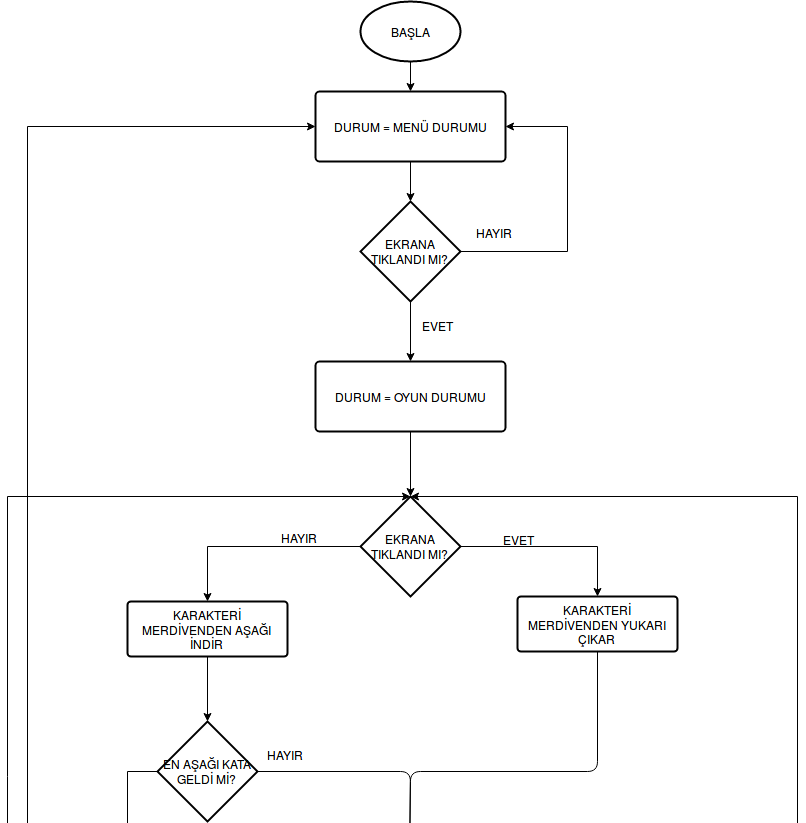
\includegraphics[width=\linewidth]{res/slice_flc_1.png}
      \end{center}

      \begin{center}
         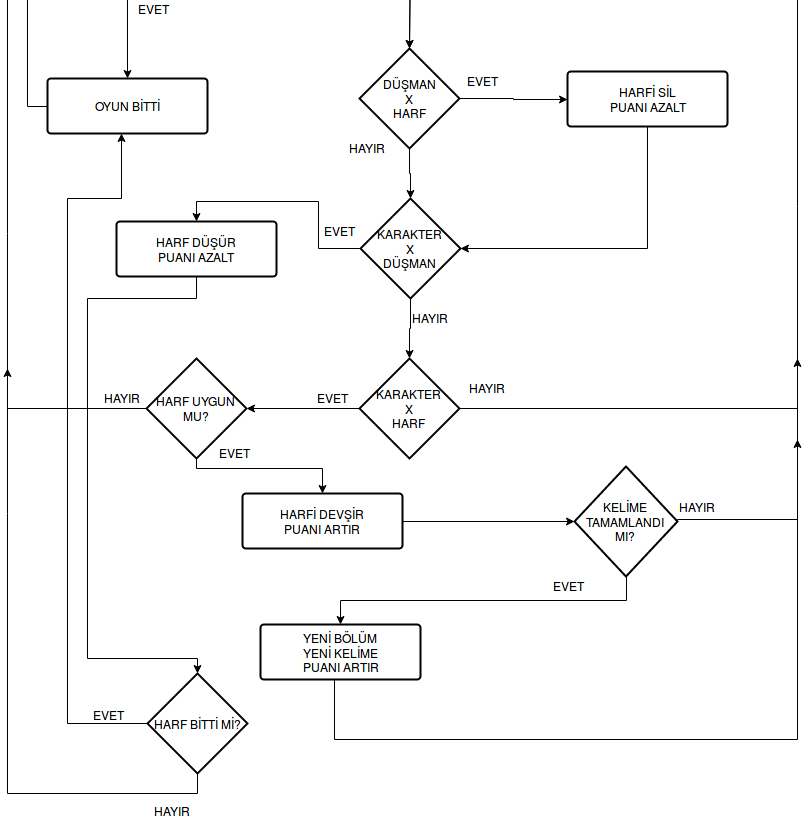
\includegraphics[width=\linewidth]{res/slice_flc_2.png}
      \end{center}

\end{document}

